

\documentclass[conference]{IEEEtran}

\usepackage{graphicx}

\newcommand{\todo}[1]{ \textbf{#1} }

% correct bad hyphenation here
\hyphenation{op-tical net-works semi-conduc-tor}


\begin{document}

\title{Variable names and use in Scratch}


% author names and affiliations
% use a multiple column layout for up to three different
% affiliations
\author{\IEEEauthorblockN{Michael Shell}
\IEEEauthorblockA{School of Electrical and\\Computer Engineering\\
Georgia Institute of Technology\\
Atlanta, Georgia 30332--0250\\
Email: http://www.michaelshell.org/contact.html}
\and
\IEEEauthorblockN{Homer Simpson}
\IEEEauthorblockA{Twentieth Century Fox\\
Springfield, USA\\
Email: homer@thesimpsons.com}
\and
\IEEEauthorblockN{James Kirk\\ and Montgomery Scott}
\IEEEauthorblockA{Starfleet Academy\\
San Francisco, California 96678--2391\\
Telephone: (800) 555--1212\\
Fax: (888) 555--1212}}

% conference papers do not typically use \thanks and this command
% is locked out in conference mode. If really needed, such as for
% the acknowledgment of grants, issue a \IEEEoverridecommandlockouts
% after \documentclass

% for over three affiliations, or if they all won't fit within the width
% of the page, use this alternative format:
% 
%\author{\IEEEauthorblockN{Michael Shell\IEEEauthorrefmark{1},
%Homer Simpson\IEEEauthorrefmark{2},
%James Kirk\IEEEauthorrefmark{3}, 
%Montgomery Scott\IEEEauthorrefmark{3} and
%Eldon Tyrell\IEEEauthorrefmark{4}}
%\IEEEauthorblockA{\IEEEauthorrefmark{1}School of Electrical and Computer Engineering\\
%Georgia Institute of Technology,
%Atlanta, Georgia 30332--0250\\ Email: see http://www.michaelshell.org/contact.html}
%\IEEEauthorblockA{\IEEEauthorrefmark{2}Twentieth Century Fox, Springfield, USA\\
%Email: homer@thesimpsons.com}
%\IEEEauthorblockA{\IEEEauthorrefmark{3}Starfleet Academy, San Francisco, California 96678-2391\\
%Telephone: (800) 555--1212, Fax: (888) 555--1212}
%\IEEEauthorblockA{\IEEEauthorrefmark{4}Tyrell Inc., 123 Replicant Street, Los Angeles, California 90210--4321}}




% use for special paper notices
%\IEEEspecialpapernotice{(Invited Paper)}




% make the title area
\maketitle

% As a general rule, do not put math, special symbols or citations
% in the abstract
\begin{abstract}
The abstract goes here.
\end{abstract}

% no keywords




% For peer review papers, you can put extra information on the cover
% page as needed:
% \ifCLASSOPTIONpeerreview
% \begin{center} \bfseries EDICS Category: 3-BBND \end{center}
% \fi
%
% For peerreview papers, this IEEEtran command inserts a page break and
% creates the second title. It will be ignored for other modes.
\IEEEpeerreviewmaketitle



\section{Introduction}
\todo{Do we want to do just variables or also functions and signals?}

\section{Results - replication ICPC}

\subsection{Distribution of lengths}

Figure \ref{fig:distribution_of_lengths} shows the distribution of lengths in the corpus.

\begin{figure}
  \begin{center}
  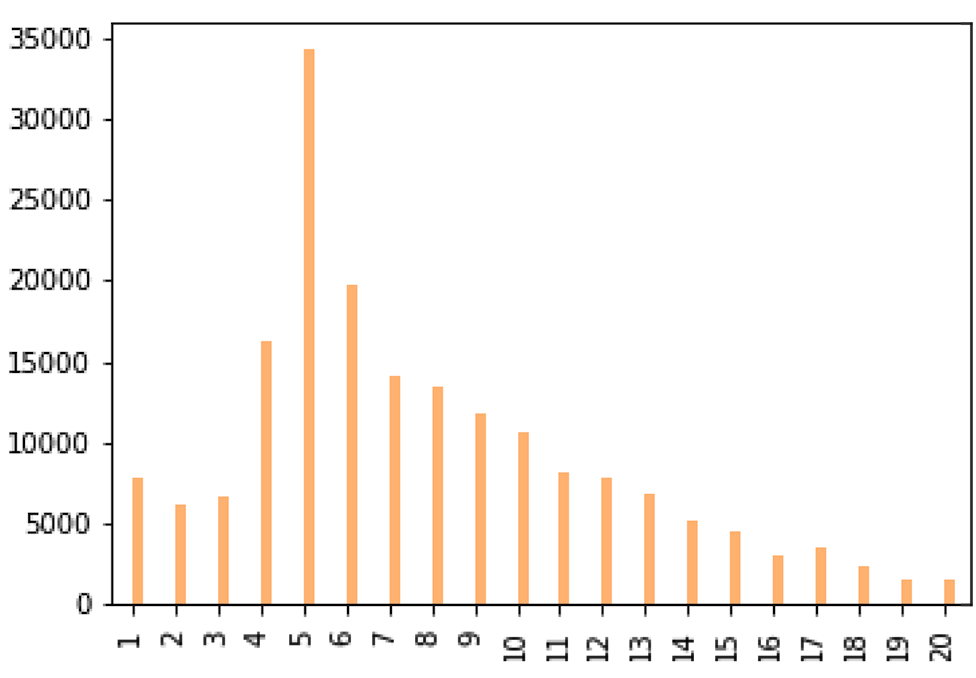
\includegraphics[width=\columnwidth]{fig/distribution_of_lengths}
  \caption{Total occurrence of variables of different lengths}
  \label{fig:distribution_of_lengths}
  \end{center}
\end{figure} 

\todo{we could sample some 5 letter identifiers here to see what they usually look like since they are an interesting peak?}

\todo{in the ICPC paper the diagram goes to 20 and then just has 20+ we could do that too?}

\subsection{One letters}

Figure \ref{fig:one_letter_occurrence} shows the distribution of variables of one letter in the corpus.

\begin{figure}
  \begin{center}
  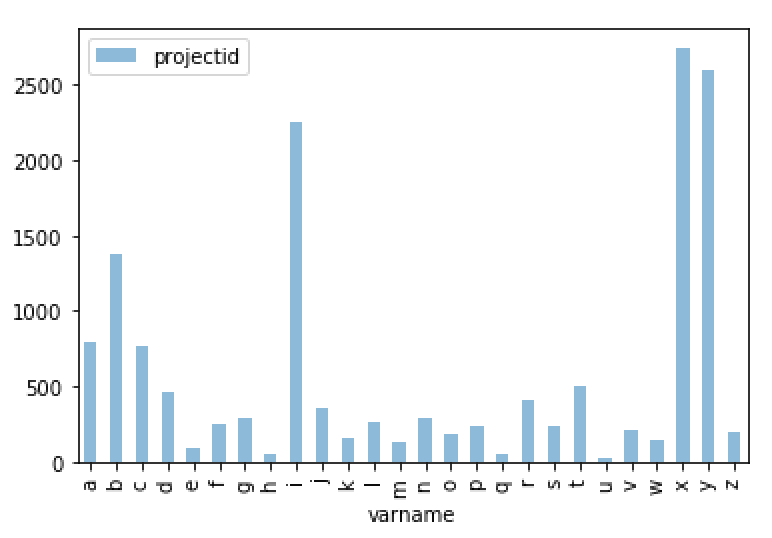
\includegraphics[width=\columnwidth]{fig/one_letter_occurrence}
  \caption{Total occurrence of variables of one letter}
  \label{fig:one_letter_occurrence}
  \end{center}
\end{figure} 

Scratch is not a typed language, variables can contain strings or numbers without declarations or casting. However, we can infer the types by attempting to cast them to a float or an int. As such we did obtain types, allowing us to compare to the ICPC paper.

Figure \ref{fig:one_letter_type} shows the distribution of variables of one letter in the corpus.

\todo{here we can reflect on the differences with "real" languages and the prevalence of ints.}

\begin{figure}
  \begin{center}
  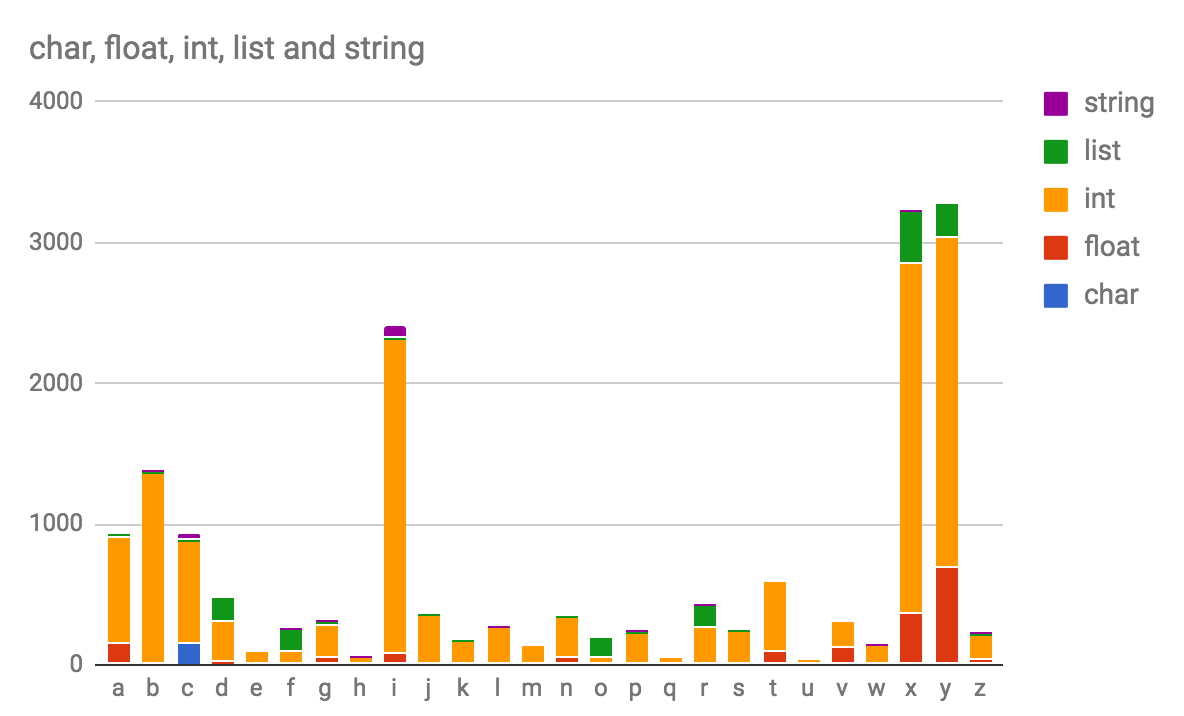
\includegraphics[width=\columnwidth]{fig/one_letter_type}
  \caption{Inferred types for variables of one letter}
  \label{fig:one_letter_type}
  \end{center}
\end{figure} 



\section{Results - Scratch specific}
\subsection{Use of spaces in variable names}

Contrary to most textual programming languages, Scratch allows users to use spaces in variable names. This is quite commonly used, about 30.000 projects use one or more variables with a space in it, versus 60.000 that use only space-free variable names. Figure \ref{fig:number_of_spaces} shows the distribution of spaces in variable names. We have found that many introductory Scratch programming materials demonstrate the use of space free variables, and that children---and adults---that already have programming experience deem the use of spaces in variables as non-natural, even though arguable `number of apples' is more natural that `nApples'.

\begin{figure}
  \begin{center}
  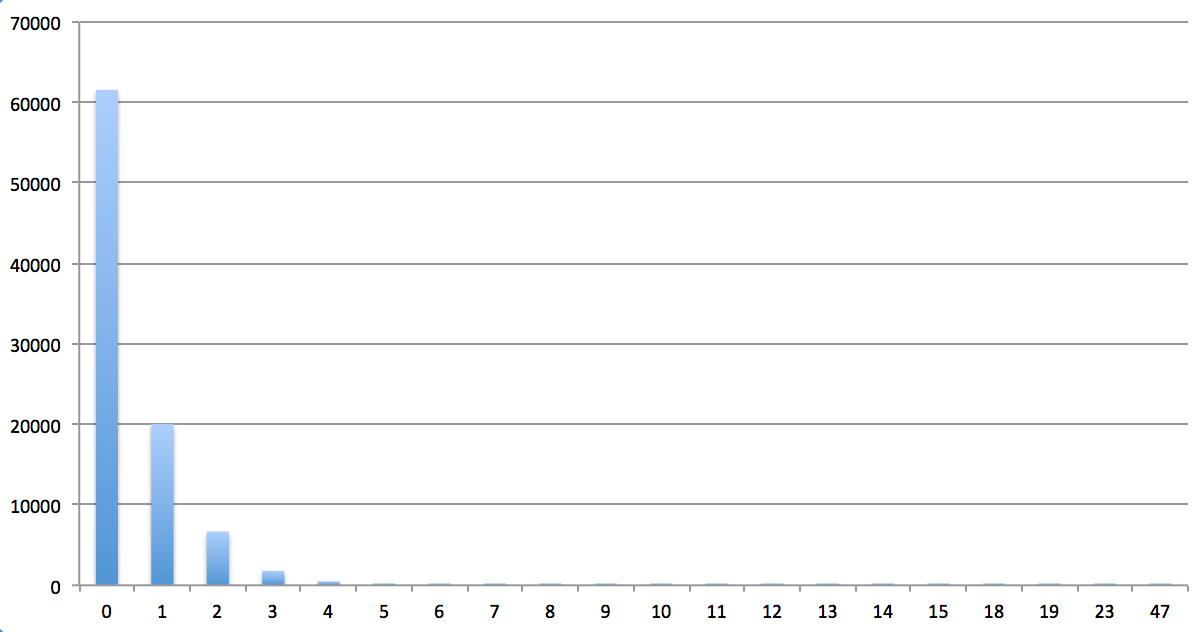
\includegraphics[width=\columnwidth]{fig/number_of_spaces}
  \caption{Number of spaces in variable names}
  \label{fig:number_of_spaces}
  \end{center}
\end{figure} 

\subsection{Use of non-letter variable names}
In addition to spaces in variable names, Scratch even allows the use of numbers and even floating point numbers as variables. We found 718 projects with integer variable names and 19 with floating point names. While their use is rare, we manually examined some projects and numbers are used in interesting and clever ways.

\todo{here we can show the tic tac toe example}

\section{Conclusion}
The conclusion goes here.




% conference papers do not normally have an appendix


% use section* for acknowledgment
\section*{Acknowledgment}


The authors would like to thank...





% trigger a \newpage just before the given reference
% number - used to balance the columns on the last page
% adjust value as needed - may need to be readjusted if
% the document is modified later
%\IEEEtriggeratref{8}
% The "triggered" command can be changed if desired:
%\IEEEtriggercmd{\enlargethispage{-5in}}

% references section

% can use a bibliography generated by BibTeX as a .bbl file
% BibTeX documentation can be easily obtained at:
% http://mirror.ctan.org/biblio/bibtex/contrib/doc/
% The IEEEtran BibTeX style support page is at:
% http://www.michaelshell.org/tex/ieeetran/bibtex/
%\bibliographystyle{IEEEtran}
% argument is your BibTeX string definitions and bibliography database(s)
%\bibliography{IEEEabrv,../bib/paper}
%
% <OR> manually copy in the resultant .bbl file
% set second argument of \begin to the number of references
% (used to reserve space for the reference number labels box)
\begin{thebibliography}{1}

\bibitem{IEEEhowto:kopka}
H.~Kopka and P.~W. Daly, \emph{A Guide to \LaTeX}, 3rd~ed.\hskip 1em plus
  0.5em minus 0.4em\relax Harlow, England: Addison-Wesley, 1999.

\end{thebibliography}




% that's all folks
\end{document}


